\documentclass{article} % For LaTeX2e
\usepackage{nips14submit_e,times}
\usepackage{amsmath}
\usepackage{amsthm}
\usepackage{amssymb}
\usepackage{mathtools}
\usepackage{hyperref}
\usepackage{url}
\usepackage{algorithm}
\usepackage[noend]{algpseudocode}
%\documentstyle[nips14submit_09,times,art10]{article} % For LaTeX 2.09

\usepackage{graphicx}
\usepackage{caption}
\usepackage{subcaption}

\def\eQb#1\eQe{\begin{eqnarray*}#1\end{eqnarray*}}
\def\eQnb#1\eQne{\begin{eqnarray}#1\end{eqnarray}}
\providecommand{\e}[1]{\ensuremath{\times 10^{#1}}}
\providecommand{\pb}[0]{\pagebreak}

\newcommand{\E}{\mathrm{E}}
\newcommand{\Var}{\mathrm{Var}}
\newcommand{\Cov}{\mathrm{Cov}}

\def\Qb#1\Qe{\begin{question}#1\end{question}}
\def\Sb#1\Se{\begin{solution}#1\end{solution}}

\newenvironment{claim}[1]{\par\noindent\underline{Claim:}\space#1}{}
\newtheoremstyle{quest}{\topsep}{\topsep}{}{}{\bfseries}{}{ }{\thmname{#1}\thmnote{ #3}.}
\theoremstyle{quest}
\newtheorem*{definition}{Definition}
\newtheorem*{theorem}{Theorem}
\newtheorem*{lemma}{Lemma}
\newtheorem*{question}{Question}
\newtheorem*{preposition}{Preposition}
\newtheorem*{exercise}{Exercise}
\newtheorem*{challengeproblem}{Challenge Problem}
\newtheorem*{solution}{Solution}
\newtheorem*{remark}{Remark}
\usepackage{verbatimbox}
\usepackage{listings}
\title{Multivariable Analysis:  \\
Problem Set I}


\author{
Youngduck Choi \\
CIMS \\
New York University\\
\texttt{yc1104@nyu.edu} \\
}


% The \author macro works with any number of authors. There are two commands
% used to separate the names and addresses of multiple authors: \And and \AND.
%
% Using \And between authors leaves it to \LaTeX{} to determine where to break
% the lines. Using \AND forces a linebreak at that point. So, if \LaTeX{}
% puts 3 of 4 authors names on the first line, and the last on the second
% line, try using \AND instead of \And before the third author name.

\newcommand{\fix}{\marginpar{FIX}}
\newcommand{\new}{\marginpar{NEW}}

\nipsfinalcopy % Uncomment for camera-ready version

\begin{document}


\maketitle

\begin{abstract}
This work contains solutions to the problem set I
of Multivariable Analysis 2016 at Courant Institute of Mathematical Sciences.
\end{abstract}

\bigskip

\begin{question}[1]
\hfill
\begin{figure}[h!]
  \centering
    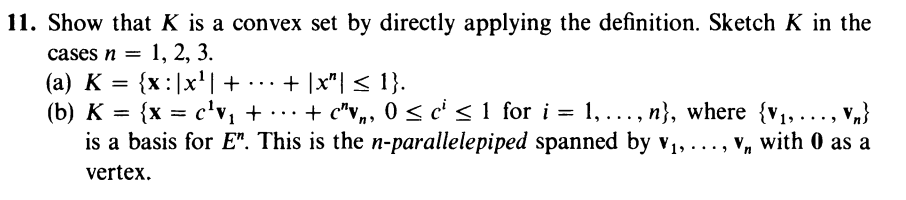
\includegraphics[width=1\textwidth]{MV-1-3-11.png}
\end{figure}
\end{question}
\begin{solution}
\textbf{(a)} Let $K = \{ x : \sum_{i=1}^{n} |x_i| \leq 1\}$, $a,b \in K$, and 
$t \in [0,1]$. Consider $l = ta + (1-t)b$ and its $l_1$ quantity, $\sum_{i=1}^{n}
|ta_i + (1-t)b_i|$. By the triangle inequality, it follows that
\eQb
\sum_{i=1}^{n} |ta_i + (1-t)b_i| &\leq& \sum_{i=1}^{n} |ta_i| + |(1-t)b_i| \\
&=& |t|\sum_{i=1}^{n} |a_i| + |1-t|\sum_{i=1}^{n} |b_i| \\
&\leq& |t| + |1-t| = 1.
\eQe 
Hence, $l \in K$.
Since $x,y,t$ were arbitrary, we have shown that $K$ is convex. 

\bigskip

\textbf{(b)} Let $K = \{ x = \sum_{i=1}^{n} c_i v_i | \>\> 0 \leq c_i \leq 1 
\>\> \text{for} \>\> i = 1,2,...,n \}$, $a = \sum_{i=1}^{n} a_i v_i
, b = \sum_{i=1}^{n} b_i v_i  \in K$, and $t \in [0,1]$. Consider 
$l = ta + (1-t)b$. It follows that
\eQb
ta + (1-t)b &=& t\sum_{i=1}^{n} a_i v_i + (1-t) \sum_{i=1}^{n} v_i \\
&=& \sum_{i=1}^{n} (ta_i + (1-t)b_i) v_i.
\eQe 
As $t,a_i,b_i, 1-t$ are all non-negative, we have $0 \leq ta_i + (1-t)b_i$.
As $0 \leq a_i, b_i \leq 1$, we obtain $ta_i + (1-t)b_i \leq t + 1-t = 1$, which 
combined with the previous inequality gives $0 \leq ta_i + (1-t)b_i \leq 1$.
Hence, $l \in K$. Since $x,y,t$ were arbitrary, we have shown that $K$ is convex. 

\hfill $\qed$
\end{solution}

\newpage

\begin{question}[2]
\hfill
\begin{figure}[h!]
  \centering
    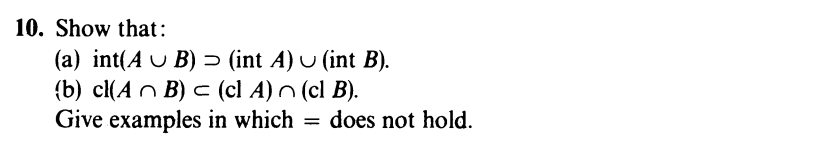
\includegraphics[width=1\textwidth]{MV-1-4-10.png}
\end{figure}
\end{question}
\begin{solution}
\textbf{(a)}
Let $x \in \text{Int} A \cup \text{Int} B$. It follows that there exists a neighborhood of 
$x$ contained in $A$ or exists a neighborhood of $x$ contained in $B$, respectively denoted 
as $U_A$ and $U_B$. If we have the existence of $U_A$, it follows that 
$x \in U_A \subset A \subset A \cup B$. Likewise, if we have the existence of $U_B$, it follows
that $x \in U_B \subset B \subset A \cup B$. Therefore, we have $x$ is an interior point of $A
\cup B$.
Since $x$ was arbitrary, we have shown that $\text{Int} A \cup \text{Int} B 
\subset \text{Int}(A \cup B)$. We now show that the equality does not hold, by providing
a counter example. Let $A = \mathbb{Q}$, $B = \mathbb{R\setminus Q}$. Then, 
$\text{int}\mathbb{R} = \mathbb{R}$ and $\text{int}\mathbb{Q} = \emptyset$ and 
$\text{int}\mathbb{R\setminus Q} = \emptyset$. Since $\mathbb{R} \not\subset
\emptyset$, we have shown that the equality does not hold. \hfill $\qed$  

\bigskip

\textbf{(b)}
Firstly, taking complements on both sides shows that the given inclusion is equivalent to
\eQb
(\text{cl}A \cap \text{cl}B)^c &\subset&
(\text{cl}(A \cap B))^c. 
\eQe
By DeMorgan's laws, we have that the above inclusion is equivalent to 
\eQb
(\text{cl}A)^c \cup (\text{cl}B)^c &\subset& (\text{cl} (A \cap B))^c.  
\eQe
Using the fact that $(\text{cl}A)^c = \text{int}(A^c)$, for any arbitrary
set $A \subset E^n$, the above inclusion is equivalent to
\eQb
\text{int} A^c \cup \text{int} B^c &\subset& \text{int}((A \cap B)^c).
\eQe
Again, by DeMorgan's laws, the above inclusion is equivalent to 
\eQb
\text{int} A^c \cup \text{int} B^c &\subset& \text{int}(A^c \cup B^c).
\eQe
As we have shown the part $(a)$ to be true, we are done. We now show that the equality 
does not hold, by providing a counter example. Let $A = \mathbb{Q}$, $B=\mathbb{R} \setminus
\mathbb{Q}$. Then, $\text{cl}(A \cap B) = \emptyset$ and $\text{cl}(A) \cap \text{cl}(B) = 
\mathbb{R}$. Since $\mathbb{R} \not\subset \emptyset$, we have shown that the equality 
does not hold. \hfill $\qed$ 
 
\end{solution}

\newpage

\begin{question}[3]
\hfill
\begin{figure}[h!]
  \centering
    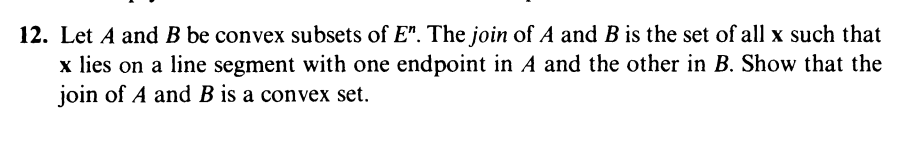
\includegraphics[width=1\textwidth]{MV-1-5-12.png}
\end{figure}
\end{question}
\begin{solution}
Let $\text{join}(A,B)$ be the join of $A$ and $B$, $\lambda \in [0,1]$,
and $x_1, x_2 \in \text{join}(A,B)$. Consider $\lambda x_1 + (1-\lambda)x_2$.
It follows that
\eQb
\lambda x_1 + (1-\lambda)x_2 &=& \lambda (t_1 a_1 + (1-t_1)b_1) + (1-\lambda)
(t_2 a_2 + (1-t_2)b_2),
\eQe
for some $a_1, a_2 \in A$, $b_1, b_2 \in B$, and $t_1, t_2 \in [0,1]$. 
\end{solution}

\newpage

\begin{question}[4]
\hfill
\begin{figure}[h!]
  \centering
    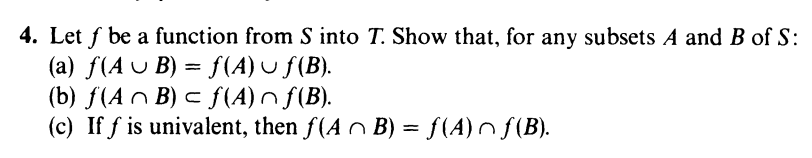
\includegraphics[width=1\textwidth]{MV-2-1-4.png}
\end{figure}
\end{question}
\begin{solution}
We first establish a trivial, yet central lemma: if $A \subset B$, then $f(A) \subset f(B)$.
We proceed with a short proof of it for sake of completeness.  
Let $y \in f(A)$. Then, there exists $x \in A$ such that $f(x) = y$. As $A \subset B$, 
we have $x \in B$, and $f(x) = y \in f(B)$. hence, the lemma is true.

\textbf{(a)}
Firstly, by the lemma, we have that $f(A) \subset f(A \cup B)$ and $f(B) \subset f(A \cup B)$.
It follows that $f(A) \cup f(B) \subset f(A \cup B)$. Conversely, 
let $y \in f(A \cup B)$. Then, there exists $x \in A \cup B$ such that $f(x) = y$. 
If $x \in A$, then $f(x) = y \in f(A)$. Likewise if $x \in B$, then $f(x) = y \in f(B)$. Hence,
$y \in f(A) \cup f(B)$. Since $y$ was arbitrary, it follows that $f(A \cup B) \subset 
f(A) \cup f(B)$. 
This completes
the proof of $f(A \cup B) = f(A) \cup f(B)$.  

\bigskip

\textbf{(b)} By the lemma, we have
\eQb
f(A \cap B) \subset f(A) \> \> \text{ and } \> \> f(A \cap B) \subset f(B).
\eQe 
It follows that $f(A \cap B) \subset f(A) \cap f(B)$. 

\bigskip

\textbf{(c)} With the additional assumption of injectivity, we wish to establish 
$f(A) \cap f(B) \subset  f(A \cap B)$. This will suffice, as we have established the reverse
inclusion for a general function in part $(b)$. Let $y \in f(A) \cap f(B)$. Then, by the
injectivity of $f$, there exists a unique $x \in S$ such that $f(x) = y$. As $y \in f(A)$ and
$y \in f(B)$, it follows that $x \in A \cap B$. Hence, $f(x) = y \in f(A \cap B)$. We have shown 
that if $f$ is injective, we have $f(A \cap B)  = f(A) \cap f(B)$.
\hfill $\qed$ 
   
  
\end{solution}

\newpage

\begin{question}[5]
\hfill
\begin{figure}[h!]
  \centering
    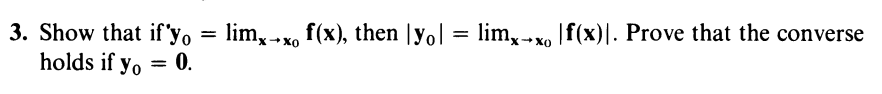
\includegraphics[width=1\textwidth]{MV-2-2-3.png}
\end{figure}
\end{question}
\begin{solution} 
Before proceeding to the main part of the proof, we prove the following lemma, which
is a mere consequence of the triangle inequality: Let 
$x,y \in E^n$. Then, $||x|-|y|| < |x - y|$. The proof is as follows: Let $x,y \in E^n$.
Then, by the triangle inequality, we obtain
\eQb
|x| &=& |x - y + y| \\
&\leq& |x - y| + |y|. 
\eQe
By subtracting both sides with $|y|$, we have $|x| - |y| \leq |x - y|$. By symmetry, we further 
obtain $|y| - |x| \leq |x-y|$, thereby showing that $||x| -|y|| < |x - y|$ as required.

\bigskip 

We now proceed with the main part of the proof.
Assume that $y_0 = \lim_{x \to x_0} f(x)$. Then, by definition, for every $\epsilon > 0$,
there exists $\delta > 0$ such that $|f(x) - y_0| < \epsilon$ whenever $0 < |x - x_0| < \delta$.
Fix $\epsilon > 0$. Let $\delta > 0$ be chosen such that
$|f(x) - y_0| < \epsilon$ whenever $0 < |x - x_0 | < \delta$, which exists by the assumption.
But, by the lemma, whenever $0 < |x - x_0| < \delta$, we have
\eQb
||f(x)| - |y_0|| &\leq& |f(x) - y_0| < \epsilon.
\eQe 
Since $\epsilon$ was arbitrary, we have shown that $|y_0| = \lim_{x \to x_0} |f(x)|$.
 
\end{solution}

\newpage

\end{document}
